
\documentclass[review]{elsarticle}

\usepackage{amsmath}
\usepackage[hidelinks]{hyperref}
\hypersetup{pdfauthor={Ricky Gole and Jamell Dacon},
  pdfsubject={Journal of Biomedical Informatics},
  pdfkeywords={weak supervision, evaluation methodology, annotation quality,
    clinical natural language processing, pre-registration, Matthews correlation}}
\usepackage{lineno}
\usepackage{float}
\makeatletter
\def\ps@pprintTitle{%
  \let\@oddhead\@empty
  \let\@evenhead\@empty
  \def\@oddfoot{}%
  \let\@evenfoot\@oddfoot}
\makeatother

\journal{Journal of Biomedical Informatics}

\begin{document}
\linenumbers

\begin{frontmatter}

\title{Attainable agreement before scoring: what a weak-supervision stage's
margins can and cannot certify}

\author[a]{Ricky Gole\corref{cor1}}
\ead{rickygole32@gmail.com}
\author[a]{Jamell Dacon}
\ead{jamell.dacon@morgan.edu}
\cortext[cor1]{Corresponding author}
\address[a]{Morgan State University, 1700 East Cold Spring Lane, Baltimore,
MD 21251, United States}

\begin{abstract}
\textbf{Objective.} A weak-supervision labelling stage is promoted on an
agreement figure computed on a small adjudicated set, beside some comparator
but not against chance. We ask what that establishes.

\textbf{Methods.} We coded how 37 clinical and biomedical weak-supervision
papers evaluate their labelling stage. We specify a check for whether an
instrument reads a stage only through its marginals, and apply $\phi_{\max}$,
the margin-constrained maximum of the Matthews correlation. Pre-registered demonstrations follow on SNLI and 253 adjudicated
clinical pairs.

\textbf{Results.} On the clinical set three marginal counts fix the attainable
ceiling at 0.0818, which needs no item-level gold labels and could have been
published before the join. The stage reached 0.0243. A hypergeometric
feasibility gate of our own construction reduced to a function of its flag
count. One threshold reproduced its verdicts on the 24 synthetic labellers
exactly, and on the pooled 31 with two disagreements. The failure set has a
second branch at zero flags. It passed 19 labellers of which 12 produced failing
students. Of the 37, none reported a labeller-level minimum detectable effect,
none tested its labeller against chance, and 17 omitted the gold positive count.
A rival baseline built as a stronger comparator carries no out-of-sample
information, so the non-separation claim is withdrawn. A further pre-registration tested our
recommendation to report that coefficient as a fraction of its ceiling. The
ratio ranked worse on our grid by 0.0897 against a registered 0.05 margin, so we
withdraw it.

\textbf{Conclusion.} A certification instrument can be principled in derivation
and still read a stage only through its marginals. Two readings are withdrawn
under their pre-registered rules and one procedural failure is disclosed.
Compute the attainable ceiling from three counts and publish it before the join.
Report it; do not gate on it or substitute the ratio for it.
\end{abstract}

\begin{keyword}
weak supervision \sep evaluation methodology \sep annotation quality \sep
clinical natural language processing \sep pre-registration \sep Matthews correlation
\end{keyword}

\end{frontmatter}

\section{Introduction}
\label{sec:intro}

Programmatic weak supervision is the default route to training labels at clinical
scale: a rule set, an ontology walk, or a prompted language model emits noisy
labels over a large unlabelled pool, and a student model is distilled from them
\cite{ratner2016dataprogramming,ratner2017snorkel,hinton2015distilling,fries2021trove,dunnmon2020crossmodal}.
Expert annotation is slow and the phenomena are rare, so the pipeline converts
rule writing into labels at scale \cite{weiskopf2013quality,henry2020n2c2}. That is where the methodological risk sits: the weak labeller is an instrument
never itself measured against the standard it replaces
\cite{jacobs2021measurement,pangakis2023validation}.

How that instrument is certified has not been characterised. We coded 37 such
papers from full text (Section~\ref{sec:survey-method}); in that sample three specific
checks are absent.
None reported a
minimum detectable effect for its labeller evaluation, none tested the labeller
against a chance or zero-skill null, and none stated a labeller-level null
hypothesis. Seventeen also did not report the number of gold positives.

\paragraph{The gap}
Several literatures hold the ingredients of a stronger standard, none routinely
applied to the labelling stage: negative controls
\cite{lipsitch2010negative}, partial-input baselines
\cite{poliak2018hypothesis,gururangan2018artifacts}, control tasks against a
randomised target \cite{hewitt2019control}, data randomisation
\cite{adebayo2018sanity}, the label-noise literature
\cite{frenay2014labelnoise,northcutt2021labelerrors,fogliato2020fairness}, and
reporting guidance that asks for explicit accounting of such threats
\cite{collins2024tripodai,sculley2015debt}. A separate literature already settles what a marginal can establish: the
Matthews correlation on a $2\times2$ confusion matrix is the phi coefficient,
whose margin-constrained maximum $\phi_{\max}$ is classical
\cite{cureton1959phimax,guilford1965phi}. Weak-labeller evaluation cites none of it.

\paragraph{A method of methods, not a new model}
We claim no new classifier, no advance over the state of the art and no new
bound. The contribution is a method of methods: which existing results to apply,
in what order, and why. Three properties of the problem space drive the choice.
Prevalence is very low, 4.74\% here, which leaves ranking statistics with poor
resolution and makes it easy to operate at a flag rate far from the prevalence.
It is that gap, not the low prevalence, that collapses attainable agreement
(Section~\ref{sec:res-ceiling}). Gold comes from one annotator, so label uncertainty can only be bounded
analytically. And the evaluation items were selected by a procedure, so a
comparator built from their metadata must be cross-fitted
(Section~\ref{sec:res-rival}).

\paragraph{What a marginal cannot certify}
A certification instrument can look principled and still read the data only
through the stage's \emph{marginals}. A gate computed from the pilot size $N$,
the gold positive count $K$ and the flag count $n$, with $N$ and $K$ fixed across
the labellers compared, is a function of $n$ alone, whatever its derivation. Its
description does not settle this; evaluating the verdict function at every
attainable input does. Two consequences follow, neither new
as mathematics: the instrument is bounded by $\phi_{\max}$ at those margins, and
it cannot distinguish a labeller from any other presenting the same three counts.
The Dutch Draw baseline \cite{vandebijl2024dutchdraw,pries2023optimalbaseline} is
built on this principle. We report the measured cost of overlooking it.
Table~\ref{tab:significance} summarises the contribution.

\begin{table}[H]
\centering
\caption{Statement of Significance.}
\label{tab:significance}
\footnotesize
\begin{tabular}{@{}p{0.30\textwidth}p{0.64\textwidth}@{}}
\hline
\textbf{Problem or Issue} & Weak supervision is the standard route to training labels for rare clinical events. How its labelling stage is certified has not been characterised. \\[4pt]

\textbf{What is Already Known} & The Matthews correlation on a $2\times2$ table is the phi coefficient, whose margin-constrained maximum $\phi_{\max}$ is classical \cite{cureton1959phimax,guilford1965phi}. Neither is connected to weak-labeller evaluation. \\[4pt]

\textbf{What this Paper Adds} & $\phi_{\max}$ as a quantity to publish before scoring: three counts fixed a clinical stage's attainable maximum at 0.0818 against an observed 0.0243. Also a check for whether a certification instrument only re-reads a statistic the stage already emits, and a pre-registered gate that reduced to its own flag count while passing 19 labellers, 12 of whose students failed. \\[4pt]

\textbf{Who would benefit from the new knowledge in this paper} & Developers and reviewers of clinical weak-supervision pipelines, who can compute the ceiling from three counts and publish it before scoring. \\
\hline
\end{tabular}
\end{table}

\section{Related Work}
\label{sec:related}

\paragraph{Weak supervision and its certification step}
Data programming and its successors combine noisy labelling functions into a
probabilistic training label
\cite{ratner2016dataprogramming,ratner2017snorkel,zhang2022wssurvey}; distant
supervision does so with a knowledge base \cite{mintz2009distant}; clinical work
extends both to ontology-driven and cross-modal settings
\cite{fries2021trove,dunnmon2020crossmodal}, with distillation supplying the
second half \cite{hinton2015distilling}. Prompted models are now used directly as
annotators, with mixed evidence on substitutability
\cite{gilardi2023chatgpt,pangakis2023validation} and design-based corrections
for downstream inference \cite{egami2023surrogates}. The paradigm assumes a labelling
function above chance contributes usable signal, aggregation absorbing the rest:
reasonable with many functions, fragile when one function is the whole stage
and the gold set is small.

\paragraph{Control baselines}
Control tasks report probe selectivity against a randomised target
\cite{hewitt2019control,belinkov2022probing}. Hypothesis-only baselines showed a
model reading half the input achieves much of full-input accuracy
\cite{poliak2018hypothesis,gururangan2018artifacts}, and heuristic probes made
the same point for inference-specific shortcuts \cite{mccoy2019hans}. The general
phenomenon is shortcut learning \cite{geirhos2020shortcut}, whose clinical instance is a model reading the scanner rather than the disease
\cite{zech2018generalization,kaufman2012leakage}. Each controls against one named threat. The rival
check asks for a comparator defined by a resource constraint: the best score
obtainable from information the labeller never read as text.

\paragraph{Attainability limits}
Matthews correlation and Cohen's $\kappa$ are bounded by their marginals
\cite{matthews1975mcc,cohen1960kappa}, long documented as the kappa paradoxes
\cite{feinstein1990paradoxes,cicchetti1990resolving,byrt1993pabak}, and the
margin-constrained maximum of phi is classical
\cite{cureton1959phimax,guilford1965phi}. Which coefficient suits an imbalanced
problem has a literature of its own
\cite{chicco2020mcc,chicco2021mccbalanced,saito2015prcurve,delgado2019kappa},
and detectable effect size is likewise bounded \cite{hanley1982meaning}. Certifying by a tail probability on a count is
standardised in acceptance sampling \cite{dodge1929sampling} and pilot-trial
progression criteria \cite{lewis2021progression}. Under fixed margins such a
test is the closed form of a label-permutation test
\cite{ojala2009permutation,combrisson2015chance}. The Dutch Draw
\cite{vandebijl2024dutchdraw,pries2023optimalbaseline} is a published baseline
whose statistic is a function of the margins alone. None of this is connected to
weak-labeller evaluation. The
bound is available. In the 37 we coded, publishing it before scoring is not.

\section{Methods}
\label{sec:method}

\subsection{Setting and notation}

A weak-supervision stage comprises a labeller $L$ mapping an item $x$ to a flag
$\ell(x) \in \{0,1\}$ or a graded score $g(x)$, run over a pool $\mathcal{P}$.
A student $S$ is trained on $\{(x,\ell(x)) : x \in \mathcal{P}\}$. The
adjudicated gold set holds $N$ items with $K$ positives, of which $L$ flags $n$. A \emph{certification} is a decision to promote the stage: to use its labels
downstream or build a claim on its score. Where a statistic is
already compared to chance, the checks below add to that comparison; in the
sample of Section~\ref{sec:survey} that comparison is never made, and they
stand alone. The Matthews
correlation on a $2\times2$ confusion matrix is the phi coefficient. Its
margin-constrained maximum is classical in psychometrics as $\phi_{\max}$
\cite{cureton1959phimax,guilford1965phi}; in confusion-matrix notation it is
obtained by placing every gold positive that fits inside the flagged set:
\begin{equation}
\mathrm{TP}^{\star} = \min(n,K), \quad
\mathrm{FP}^{\star} = n - \mathrm{TP}^{\star}, \quad
\mathrm{FN}^{\star} = K - \mathrm{TP}^{\star}, \quad
\mathrm{TN}^{\star} = N - n - \mathrm{FN}^{\star},
\label{eq:ceiling}
\end{equation}
with $\mathrm{MCC}_{\max} = \mathrm{MCC}(\mathrm{TP}^{\star}, \mathrm{FP}^{\star},
\mathrm{FN}^{\star}, \mathrm{TN}^{\star})$, and $\mathrm{MCC}=0$ when a
denominator factor vanishes. The arrangement is explicit, so the bound is
attained and tight.

\subsection{Check 1: collapse}
\label{sec:check-collapse}

The \emph{a priori} form of the check is a code reading: list the verdict
function's arguments. If the function reads the data only through a vector of
marginals with all but one component fixed across the units compared, the
verdict is a function of that component. The \emph{empirical} form compares verdict vectors. Let $V_i$ be the verdict on
unit $i$ and $t_i$ a candidate statistic.
Evaluate the instrument at every attainable value of $t$ to obtain its failure
set, then report (i) the threshold on $t$ whose verdicts come closest to $V$,
with the disagreement count, and (ii) the best Youden $J$ over all thresholds. Step (i) is the comparison that matters because it involves no selection. Zero disagreements over units spanning the attainable range of $t$ establishes
the equivalence on that range. Where the failure set is not a single interval,
as in our own demonstration, a grid omitting part of it can show zero
disagreements while the equivalence fails elsewhere; we report both arms. Step (ii) is diagnostic only: its threshold is chosen in sample, so its value
is an optimistic bound. Screening operating characteristics cannot substitute: an instrument can have
perfect specificity and still be redundant.

\subsection{Check 2: rival}

Enumerate variables available to the pipeline but not to the labeller as text:
the generating rule, source section, note type, document length, position. Build the best score obtainable from each alone; the obvious candidate is the
stratum base rate $s(x) = k_{r(x)}/n_{r(x)}$. Score it on the same items as the
stage and compare with a paired test; for AUROC, DeLong's
\cite{delong1988comparing}.

Four requirements are not optional. \emph{Cross-fit the rival.} A rival estimated from the gold labels it is scored
against is optimistic, and at a small positive count that optimism can exceed
the signal.
\emph{Make the null refit it.} Holding a fitted score vector fixed while
permuting the labels it was fitted to tests the wrong hypothesis, and such a
statistic may be bounded below by its chance value.
\emph{Report the comparison's stability.} A single cross-fit is one partition, and
the verdict can move across its whole range with it, so report the distribution
over assignments.
\emph{Compute the detectability bound first.} The comparison may be unable to
return a positive answer at any attainable value. Pre-register three outcomes. A null result licenses only the statement that the
study cannot distinguish stage from rival, not that the stage carries nothing.

\subsection{Check 3: ceiling}

This check is imported apparatus and we claim no part of the bound.
Equation~\ref{eq:ceiling} is $\phi_{\max}$ in confusion-matrix notation, and the
analogous construction gives $\kappa_{\max}$. What is new is its transport to
weak-labeller evaluation, and the consequence for a whole class of screens that
this literature has not drawn.

That consequence is the check. Before scoring, record $N$, $K$ and $n$ and
compute $\mathrm{MCC}_{\max}$. Report the observed coefficient, the ceiling, and the minimum detectable effect
for every comparison the conclusion rests on, not only the one against chance
\cite{hanley1982meaning}. Publish the ceiling as context for reading the
coefficient; do not substitute the ratio for it, which
Section~\ref{sec:res-ratio} tests and finds worse. Because the ceiling depends only on marginals it
needs no item-level gold labels, only their count. It can therefore be published
once the stage has run and before its output is joined to gold. The ceiling is itself a function of $(N,K,n)$, so by the argument of
Section~\ref{sec:check-collapse} it cannot distinguish a labeller from any other
presenting the same three counts. Demonstration~1's gate is this same arithmetic
with a tail threshold, which is why we report the ceiling and
do not gate on it. At $N=253$, $K=12$ and $n=223$ it is 0.0818
both for a stage whose 223 flags contain all 12 positives and for one that
flagged 223 items at random. It is a statement about representability, never
about quality, and it binds a hard-label stage. Where the labeller emits a score,
$n$ is a free parameter. The ceiling at the observed $n$ then bounds the
operating point that was chosen rather than the labeller, and belongs beside a threshold
sweep. It is not a power calculation: power asks whether an effect of a given size is
detectable, the ceiling whether one of a useful size is representable.

\subsection{The survey of certification practice}
\label{sec:survey-method}

We coded 37 clinical and biomedical weak-supervision papers published between
2019 and 2026 \cite{fries2021trove,das2025criticalfindings,hsu2025knowledgefree,datta2023spatial,wang2019weaksupervisionparadigm,banerjee2019weaklysupervised,vidmar2025probabilistic,jeffery2024noisylabels,azzouzi2024deidentification,dong2023raredisease,wang2022ophthalmologyexam,bejan2022suicidality,shen2022lifestyle,zhang2021chestxray,danniballe2022multilabel,nogues2022weaklysemisupervised,gan2025arch,zhu2021distantlysupervised,vashishth2021medtype,eyuboglu2021multitask,cusick2021suicidalideation,kshatriya2020inhaler,gori2019patientcentered,hsieh2024genegene,agnikula2021asthmacontrol,sanyal2021recurrence,godoy2026mammography,sandlin2026decisional,algaradi2026copd,greco2026west,gao2022keyclass,irvin2019chexpert,smit2020chexbert,agrawal2022fewshot,guevara2024sdoh,yoon2023kbrefined,huemann2023nuclearmedicine}. Records were identified by keyword search of PubMed, arXiv and the ACL Anthology, with four added by known-item search. Eligibility required
programmatic weak supervision, distant supervision or model-generated labels over clinical or
biomedical text, and machine-readable full text. Each paper was coded for whether
the labelling stage was evaluated against gold at all, the comparator used, the
null tested if any, whether prevalence and the gold positive count were reported,
and whether any power or minimum-detectable-effect calculation appeared. The
search strings, dates, eligibility criteria, flow counts and the coding
instrument are released with the analysis code, as is the coded table.

This is a motivating survey and not a systematic review: it establishes a premise
with a stated sampling frame and is not offered as a headline empirical
contribution. Promotion would require a pre-registered protocol, a second coder
and a record-level screening log, none of which this sample has.

The sample is purposive and was not pre-registered. Eligibility
required machine-readable full text, so it is biased toward open access; five
candidate studies were dropped for inaccessible full text. Comparators were coded
generously, as present anywhere in the paper, which inflates comparator counts
and makes the negative findings conservative. One author coded every record by hand from the full
text, with no second rater and no agreement statistic.

\subsection{Demonstration 1: a feasibility gate on public data}
\label{sec:mat-d1}

The instrument under test is a marginal feasibility gate we constructed and
pre-registered as a screen for student failure. We are not aware of a published procedure
that certifies a weak labeller by a tail test on its flag count, so the gate is our own construction standing for that class. It is evaluated as a screening test, with gate failure as the positive result
and an unusable student as the condition.

Data are SNLI \cite{bowman2015snli}, binarised as $y=1$ iff contradiction, in
three disjoint frames at 4\% prevalence under seed 42: a 300-item pilot with 12
positives, a 5000 pool with 200, and a 10,000 test frame with 400. The
gate computes the ceiling of Equation~\ref{eq:ceiling} and the hypergeometric
floor $p_{\text{floor}} = P(X \ge \min(n,K))$ for
$X \sim \mathrm{Hypergeometric}(N,K,n)$, failing when $p_{\text{floor}} \ge 0.05$.
At $N=300$ and $K=12$ its verdict uses the pilot alone. The gate is therefore
Check 3 read through a tail threshold, and on this grid the two coincide
exactly: the failure set below is $\{n : \mathrm{MCC}_{\max}(n) \le 0.1074\}$.

There are 31 labellers. The primary arm is 24 synthetic labellers, each a pair
$(\mathrm{TPR},\mathrm{FPR})$ with TPR in $\{0.90, 0.50, 0.10, 0.04\}$ and FPR
from 0.01 to 0.97, including near-chance labellers at low flag rates, where a
marginal gate is expected to pass a useless labeller. The secondary arm
is 7 locally run open-weight models (\texttt{qwen3} at 0.6b, 1.7b, 4b, 8b and
14b, \texttt{llama3:8b}, \texttt{granite3.3:8b}) under one plain contradiction
prompt at temperature 0.

The primary student encodes premise and hypothesis with a locally run MiniLM
encoder and fits $L_2$-regularised logistic regression; a secondary uses TF-IDF. Both train on
the 5000 pool items with that labeller's labels and are scored by AUROC on the
10,000 item frame, with failure set below 0.60. The pre-registration required the primary
student's clean-label reference AUROC to exceed 0.75: MiniLM reached 0.8167 and
TF-IDF 0.6037.
Outcome A required sensitivity and positive predictive value both at or above
0.90 \emph{and} that the verdicts not be reproducible by a single threshold on
the flag-rate ratio. The kill condition forbade changing any threshold, seed,
frame, grid entry or outcome definition after the first number was seen.

\subsection{The pipeline's production labeller and detector}
\label{sec:mat-pipeline}

Two objects in Section~\ref{sec:res-ceiling} belong to the pipeline itself. The production labeller is Llama 3 8B \cite{grattafiori2024llama3}, run
locally, given each candidate's exemplar sentence pair and the identifier of the
rule that generated it, and asked for a binary judgement and a confidence value
under a fixed template with no demonstrations. It received the rule identifier;
the prompts of the 17 configurations of Section~\ref{sec:mat-d2} name no rule.
Neither that prompt nor the script that sent it was committed, so the run cannot
be repeated and its flag counts are measured but not regenerable. We report the
ceiling from them because it needs only the three marginal counts. The downstream
detector is a BiomedBERT-base pair classifier \cite{gu2021domainspecific}
fine-tuned for three epochs with AdamW at learning rate $2\times10^{-5}$ and
maximum length 160 on the 1,183-row training pool.

\subsection{Demonstration 2: a rival on a clinical instance}
\label{sec:mat-d2}

The clinical corpus is a de-identified critical care database
\cite{johnson2016mimic} accessed under a data use agreement. A pharmacist
annotated 299 candidate pairs: 12 contradictions, 241 not contradictions and 46
ambiguous. The evaluation set $\mathcal{G}_{253}$ is the 253 non-ambiguous pairs,
12 of them positive, a prevalence of 4.74\%. No second rater is available.

Seventeen configurations each cross one of three locally run models,
\texttt{llama3\discretionary{}{}{}:8b}, \texttt{granite3.3\discretionary{}{}{}:8b} and \texttt{qwen3\discretionary{}{}{}:8b}, with a prompt
wording, scored by a
graded flag log-odds. Two are determinism re-runs reproducing their AUROC to every printed digit, so
the 17 cover 15 distinct cells and must not be read as 17 independent wordings. No new inference was run: this is
reanalysis of committed per-pair score caches. The rival assigns each pair the
confirmed positive rate of its generating rule, computed on
$\mathcal{G}_{253}$ itself. The four rules cover 117, 28, 63 and 45 pairs with
3, 3, 4 and 2 confirmed positives. It reads no text, and no prompt names a rule.

Against chance we use a one-sided label-permutation test with 20,000 draws at
seed 109 and a percentile bootstrap with 10,000 draws. Against the rival
we use a paired two-sided DeLong test \cite{delong1988comparing} on the same 253
pairs. Outcome A promoted the stage if any configuration cleared the corrected
threshold above the rival; Outcome B required reporting non-separation; Outcome C covered the rival winning. No
outcome licensed dropping the check. A second pre-registration, written before
any datum of it was read, added the cross-fitting, refitting-null and
detectability analyses reported in Section~\ref{sec:res-rival}.

\section{Results}
\label{sec:results}

\subsection{Three specific checks are absent}
\label{sec:survey}

Thirty-six of the 37 papers coded report at least one comparator, most often a
simpler text model (25) or another labeller (23). Three specific checks are
nonetheless absent from all of them. None reported a minimum detectable effect
for its labeller evaluation, none tested the labeller's agreement with gold against a
zero-skill null, and none stated a labeller-level null hypothesis. Two reported a random baseline anywhere, one a majority-class baseline. Nine reported a structured-data comparator, seven of them against the
labelling stage on the same task, and in five of those seven that data
was the labeller's input or label source. Eleven reported no gold-referenced evaluation of the stage, and six evaluated
only a component or scored on the set used to tune it.

Seventeen papers did not report the number of
gold positives and fifteen did not report prevalence, so a reader of those cannot
reconstruct the chance level. That does not explain the absence. Counting
papers where the figure is derivable from other reported counts, prevalence is
recoverable in 22 of 37 and the gold positive count in 20 of 37. The test is
absent in all 37. The information is usually there; the comparison is not made. The smallest gold sets hold 5 positives at 0.83\% prevalence, 15 positives and
19 positive patients.

This changes what the paper proposes: in the sample we coded, a ceiling published
before scoring and a cross-fitted comparator are not corrections to a lenient
practice but new.

\subsection{The ceiling check on the deployed labeller}
\label{sec:res-ceiling}

The deployed clinical labeller flagged 223 of the 253
adjudicated pairs (Table~\ref{tab:controls}), a flag rate of 0.8814, against 12
gold positives. By
Equation~\ref{eq:ceiling} its Matthews correlation could not have exceeded 0.0818
whatever its judgement, because at that flag rate the confusion matrix is almost
entirely false positives by construction. Figure~\ref{fig:ceiling-curve} places that operating
point against the regime where the check is not redundant. It
reached 0.0243. The one-sided hypergeometric $p$ for its true positive count is 0.5722, and
57.11\% of 10,000 random permutations score at least as high. At these margins the statistics those papers report instead are bounded too:
precision at 0.0538 and $F_1$ at 0.1021. The ceiling required no gold labels beyond their
count and no model run. The labeller emits a score, so this bounds the
operating point it was run at, and only the marginals survive, so no sweep is
possible.
Published when the flag rate was first observed, it would have framed the
scoring as the measurement of a coefficient that could not take a useful value
at those margins.

\begin{table}[!ht]
\centering
\caption{Attainability ceiling for the pipeline's production labeller on both
adjudicated sets. The ceiling is $\phi_{\max}$ at the observed margins
\cite{cureton1959phimax,guilford1965phi} and needs only the three counts in the
first row; it is attained by the arrangement of Equation~\ref{eq:ceiling} and is
therefore tight. The 299 pair column scores the 46 ambiguous pairs as negatives;
the 253 pair column, which every reported result uses, excludes them.}
\label{tab:controls}
\small
\begin{tabular}{lrr}
\hline
Quantity & 299 pair set & 253 pair set \\
\hline
Items, gold positives, flags & 299, 12, 261 & 253, 12, 223 \\
Flag rate & 0.8729 & 0.8814 \\
Confusion cells TP/FP/FN/TN & 11/250/1/37 & 11/212/1/29 \\
Observed Matthews correlation & 0.0269 & 0.0243 \\
Marginal ceiling on Matthews correlation & 0.0780 & 0.0818 \\
One-sided hypergeometric $p$ for TP & 0.5347 & 0.5722 \\
Random joins scoring at least as high & 0.5442 & 0.5711 \\
\hline
\end{tabular}
\end{table}

\begin{figure}[!ht]
\centering
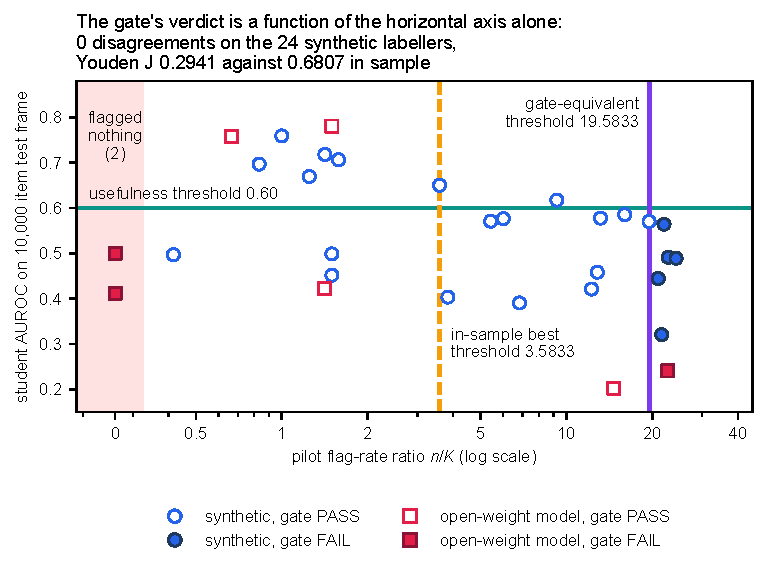
\includegraphics[width=\textwidth]{fig1}
\caption{The attainable maximum of the Matthews correlation as a function of the
flag rate, at four prevalences, computed from Equation~\ref{eq:ceiling} on a
253-item set. Each curve reaches 1 where the flag rate equals the prevalence, so
no prevalence by itself bounds the coefficient; what bounds it is the gap between
the two. At the 4.74\% prevalence of this study the ceiling is 0.6893 at a flag
rate of 0.0949, 0.4496 at 0.1976 and 0.2760 at 0.3953. The shaded band is
computed, not drawn: it is the flag rates above the prevalence, 0.1225 to
0.5534, whose ceiling lies between 0.20 and 0.60, running from 0.5971 at
the left edge to 0.2005 at the right, so a reported coefficient of 0.2 is a
third of the attainable maximum at one edge and all of it at the other. The marked point is the deployed clinical stage, which lies far outside the
band and is visibly degenerate from its flag rate without any coefficient at
all.}
\label{fig:ceiling-curve}
\end{figure}

\subsection{A gate with perfect specificity that reads one number}
\label{sec:res-collapse}

Table~\ref{tab:gate} reports the gate as a screening test. In the primary reading
(24 synthetic labellers, MiniLM student, usefulness threshold 0.60) it failed 5 labellers and all 5 of their students failed. It passed 19, of which 12 still produced a
failing student, a fraction of 0.6316. Sensitivity was 0.2941 against the
pre-registered requirement of 0.90, so the registered outcome is C, not
validated. The 0.70-threshold arm does not move the conclusion: sensitivity 0.2381, 16 of
19 passed labellers still failing. Pooling the 7 real models with the 24
synthetic gives 0.3636 and 14 of 23 still failing.

\begin{table}[!ht]
\centering
\caption{The feasibility gate as a screening test, and the raw flag-rate ratio as
its substitute. Positive test result is ``the gate fails the labeller''; the
condition is ``the distilled student's test AUROC is below the usefulness
threshold''. The primary reading is the first row; 2x2 cells are given as gate
fail/student failed, gate fail/student useful, gate pass/student failed, gate
pass/student useful. Every MiniLM gate row has specificity and positive
predictive value of 1.0000 and sensitivity never above 0.37 on any arm containing the synthetic grid,
and the TF-IDF row has no defined specificity because no student in it cleared
the threshold: the gate never wrongly condemns a labeller and almost never
condemns one. In the primary reading the raw ratio at the gate-equivalent
threshold reproduces the gate's verdicts with zero disagreements, so the gate
carries no information beyond the pilot flag count. The last row's
threshold was selected in sample over all attainable thresholds and is an
optimistic bound, not a validated operating point.}
\label{tab:gate}
\footnotesize
\setlength{\tabcolsep}{3.5pt}
\resizebox{\textwidth}{!}{%
\begin{tabular}{llrrrrrr}
\hline
Arm & Instrument & 2x2 cells & Sens. & Spec. & PPV & NPV & $J$ \\
\hline
24 syn, MiniLM, .60 & gate & 5/0/12/7 & 0.2941 & 1.0000 & 1.0000 & 0.3684 & 0.2941 \\
24 syn, MiniLM, .70 & gate & 5/0/16/3 & 0.2381 & 1.0000 & 1.0000 & 0.1579 & 0.2381 \\
31 pooled, MiniLM, .60 & gate & 8/0/14/9 & 0.3636 & 1.0000 & 1.0000 & 0.3913 & 0.3636 \\
7 real, MiniLM, .60 & gate & 3/0/2/2 & 0.6000 & 1.0000 & 1.0000 & 0.5000 & 0.6000 \\
24 syn, TF-IDF, .60 & gate & 5/0/19/0 & 0.2083 & n/a & 1.0000 & 0.0000 & n/a \\
\hline
24 syn, MiniLM, .60 & ratio at 19.5833 & 5/0/12/7 & 0.2941 & 1.0000 & 1.0000 & 0.3684 & 0.2941 \\
24 syn, MiniLM, .60 & ratio, best in samp. & 14/1/3/6 & 0.8235 & 0.8571 & 0.9333 & 0.6667 & 0.6807 \\
\hline
\end{tabular}}
\end{table}

The a priori collapse check predicts this, and this form of the finding needs no
data at all. With $N=300$ and $K=12$ fixed across all 31 labellers the gate's
internal quantities are functions of the flag count alone, so the verdict is a
function of $n$. Evaluating $p_{\text{floor}}$ at every flag count from 0 to 300
gives the failure set exactly: the point 0 together with the upper tail from
235 to 300. The empirical form corroborates it with a scope that must be stated.
Predicting student failure when the flag-rate ratio $n/K$ reaches 19.5833, the
gate's own boundary rather than a fitted value, reproduces the gate's verdict on
all 24 primary-arm labellers with zero disagreements and the identical
$2\times2$ of 5/0/12/7. The pooled arm contains the two real models that flagged
nothing, and shows 2 disagreements, because the failure set has two branches and
no synthetic labeller flagged zero. Sweeping every threshold on that ratio, the best
Youden $J$ is 0.6807 at 3.5833 against the gate's 0.2941
(Figure~\ref{fig:collapse}), chosen in sample and so an upper bound, not an
operating point. Because the gate is the
ceiling read through a tail threshold, Table~\ref{tab:gate} also measures Check
3 used as a screen: sensitivity 0.2941 for an unusable student, beaten in sample
by the ratio itself. That is the measured reason to report the ceiling and not decide with it.

\begin{figure}[!ht]
\centering
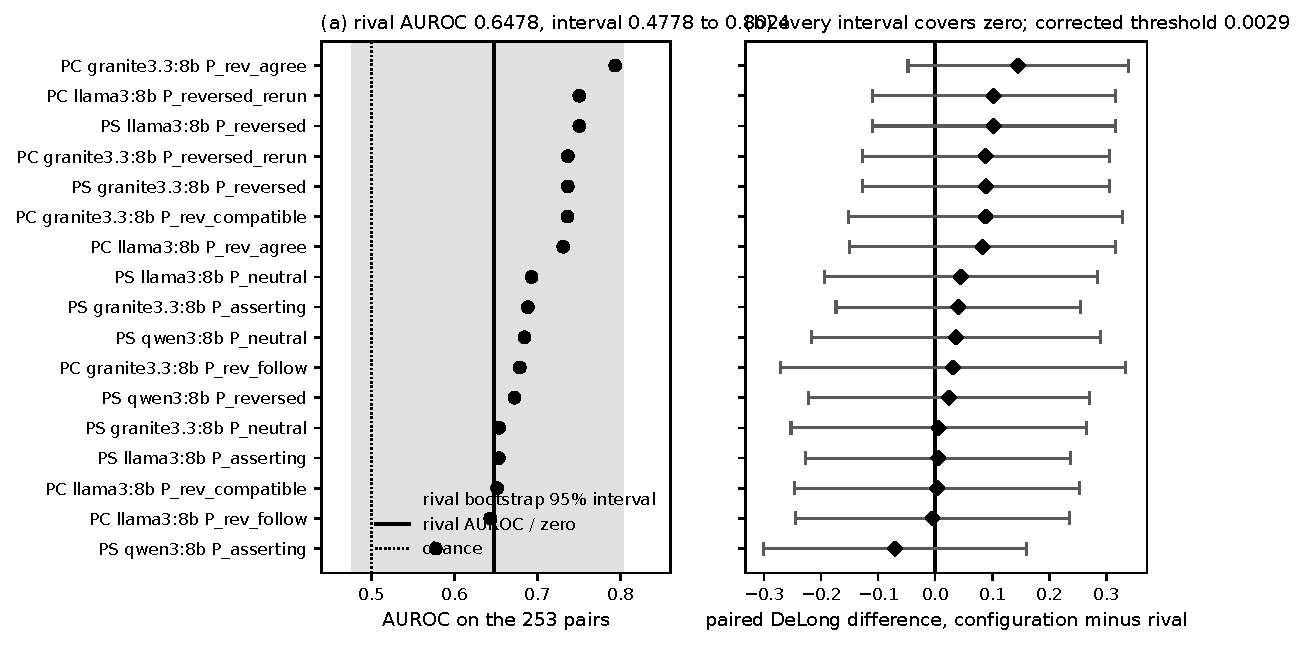
\includegraphics[width=\textwidth]{fig2}
\caption{The gate's decision boundary against the statistic it is a function of.
Each point is one of 31 labellers; the horizontal axis is the pilot flag-rate
ratio $n/K$ on a logarithmic scale, the vertical axis the distilled student's
AUROC on the 10,000 item test frame. A logarithmic axis cannot show zero, so the
two labellers that flagged nothing are drawn at the left edge, inside the shaded
band, and that tick is labelled 0; they are the failure set's second branch and
not a small ratio. The horizontal line at 0.60 is the
pre-registered usefulness threshold; the solid vertical line at 19.5833 is the
threshold on the ratio that reproduces the gate's verdicts exactly in the primary
arm; the dashed vertical line at 3.5833 is the in-sample best threshold on the
same ratio. The gate's boundary sits far to the right of where students begin to
fail, which is why its sensitivity is 0.2941, and the whole apparatus reduces to
the position of a vertical line on this axis.}
\label{fig:collapse}
\end{figure}

\paragraph{What the gate does buy}
One narrow thing. Two of the 7 real models, \texttt{qwen3:4b} and
\texttt{qwen3:8b}, flagged none of the 300 pilot items and are caught by the
failure set's zero branch. Detecting a labeller that emitted nothing saves
training compute and says nothing else. That is a sufficient condition for
hopelessness which fires almost never: defensible for an instrument, and not a
feasibility criterion.

\paragraph{The screening statistics are not estimates}
Sensitivity, specificity and the predictive values in
Table~\ref{tab:gate} are computed over 24 synthetic labellers on a grid we chose,
on an incomplete cross of TPR and FPR values. Each is a deterministic function of that composition, so a Wilson interval
\cite{wilson1927probable} would address sampling error that is not the problem:
there is no population being sampled, and the four places are exact properties
of a stated construction. With the TF-IDF student no synthetic labeller cleared
0.60, so that outcome has no variance and specificity is undefined: a screen
cannot be validated against an outcome that never varies.

\subsection{The ratio is not the statistic to report}
\label{sec:res-ratio}

A further pre-registration asked whether the observed coefficient as a fraction
of its ceiling ranks labellers by downstream usefulness better than the
coefficient itself. Over the 29 of 31 Demonstration~1 labellers with a defined
ratio, Spearman $\rho$ against the distilled student's AUROC is 0.9241 for the
raw coefficient and 0.8345 for the ratio. The difference is $-0.0897$ against a
registered margin of 0.05. The registered outcome is C, the ratio ranks worse,
and the instruction to report the observed value as a fraction of the ceiling
is withdrawn under the rule fixed before the run. Neither $\rho$ estimates a population quantity: 24 of the 29 sit on a
constructed grid, and the margin comparison is the registered decision rule on
that grid rather than an inferential test. The raw coefficient's 0.9241 is not evidence that pilot
agreement generalises, because on this grid both it and the student's AUROC are
monotone in the chosen pair of rates. An earlier pre-registration recorded, as
deciding nothing, over the 24 synthetic labellers, $\rho = 0.5310$ for the
ceiling against student AUROC and $-0.5197$ for the gate's floor probability. The
same monotonicity applies, so neither is evidence that the ceiling ranks
labellers. The registered rule was written to withdraw on this
evidence and not to adopt on it.

Nine labellers fall inside the band of Figure~\ref{fig:ceiling-curve}, where
the check is not redundant, and two meet the registered criterion. That band is computed at the clinical prevalence; the band for this 300-item
grid runs 0.1067 to 0.5100 and selects the same two. One flags 72 of 300, a rate of 0.2400, and reaches
0.3632, which is exactly its ceiling. The other flags 43, a rate of 0.1433, and
reaches 0.4505 against a ceiling of 0.4990. A reader meeting 0.3632 would call that coefficient weak; at these margins it
is the largest the table permits, which the flag rate alone does not say.
Neither labeller is rescued by that. Their distilled students reached 0.5766
and 0.6504 against the 0.60 usefulness threshold, so the one whose coefficient
attains its ceiling exactly is among the twelve the gate passed and whose
student failed. The ceiling bounds what a coefficient can represent, never whether a stage is
useful. The
qualifying criterion is itself the ratio, and at TPR 0.90 inside the band a
near-unit ratio follows from the grid, so neither case shows the criterion discriminating. Both
are synthetic: none of the seven real models lies inside the band.

\subsection{The rival baseline carries no out-of-sample information}
\label{sec:res-rival}

Two properties of a small, procedurally selected gold set govern this section: a
comparator fitted on the labels it is scored against is optimistic, and
cross-fitting leaves the verdict a function of the fold assignment.

On $\mathcal{G}_{253}$ the chance-based reading is encouraging. Of 17
configurations, 16 reject chance at 0.05 under the 20,000 draw permutation test,
6 clear the Bonferroni threshold and 12 have a bootstrap lower bound above 0.5.
The 17 contain two determinism re-runs covering 15 distinct cells, and both
duplicates fall inside the counted sets. Each figure therefore drops by two:
14 of 15,
4 at the registered divisor of 17, and 10. One further cell misses that
registered threshold by 0.0000587 and would clear a post-hoc divisor of 15; we
report the registered figure. The rule-identity prior, whose only content is which of four mining rules
produced a pair, reached AUROC 0.6478 at a permutation $p$ of 0.0367, and no
configuration separated from it under paired DeLong
(Table~\ref{tab:delong}). A pre-registered re-analysis does not sustain that.

\paragraph{Refitting the null and cross-fitting the rival}
The prior's four stratum rates are estimated from the same 12 positives it is
then scored against, and the null that produced $p = 0.0367$ holds the fitted
score vector fixed while permuting the labels it was fitted to. Refitting the
rates to each permuted draw gives $p = 0.2702$ against a null mean of 0.6182.
Cross-fitted by repeated stratified $K$-fold over 200 repeats it reaches 0.4939
at $K=5$, 2.5th to 97.5th percentile 0.3679 to 0.5668, and 0.5026 at $K=3$. Out of sample it is indistinguishable from chance, and its in-sample optimism of
0.1539 exceeds the whole above-chance portion of that value.
Leave-one-pair-out is not usable here, scoring each pair as
$(k_r - y_i)/(n_r - 1)$, a function of its own label.

\paragraph{The comparison redone against a cross-fitted rival}
On a five-fold assignment at seed 141, whose rival sits at 0.5278, all 17 cells
lie above it pointwise, 3 of the 15 distinct cells clear $p<0.05$ two-sided and
none clears the corrected threshold, the smallest $p$ being 0.003964 against
0.003333. Different pre-registrations fixed the two corrections: the chance
family at $\alpha/17$, the re-analysis at $\alpha$ over the 15 distinct cells.
Across 200 assignments that count has median 2 and a 95\% percentile interval
of \textbf{1 to 13} of 15, with a mean of 3.98 and extremes of 0 and 15. At
least one cell clears the corrected threshold in 35.5\%. The verdict ranges over the
whole scale with an arbitrary partition of the same 253 pairs, so the
reportable quantity is the distribution, not any single comparison.

The detectability bound differs by comparator. Against the in-sample rival at
0.6478, variance recomputed at the alternative with zero covariance assumed
because it was not estimated, which makes both bounds conservative, a configuration would need AUROC 0.8654 to clear
0.05 and 0.9414 corrected. Against the cross-fitted rival at 0.5278 the
strongest cell, 0.7936, cleared 0.05 and missed the corrected threshold by
0.0006 in $p$. The published floor of 0.7355 bounds the chance comparison
only.

\paragraph{Withdrawals}
We withdraw the claim that the graded scores do not separate from a
rule-identity prior, and the mechanism claim built on it. Neither is replaced: at
this gold-set size the corrected comparison supports no claim about any
configuration.

\begin{table}[!ht]
\centering
\caption{Paired DeLong comparison of 17 labeller configurations against the
rule-identity rival on the same 253 pairs with 12 positives. PS is the
prompt-sensitivity family and PC the prompt-confirmation family; $\ddagger$ marks
a determinism re-run of the row above its own family's entry, so the 17 rows
cover 15 distinct cells. $B$ marks a configuration clearing the chance threshold
corrected across configurations and $L{>}0.5$ one whose bootstrap lower bound
exceeds 0.5; over distinct cells, at the registered divisor of 17, those counts are 4 and 10. Bold marks the highest AUROC and the smallest $p$. The rival against which these
differences are computed is fitted in sample and carries no out-of-sample
information (Section~\ref{sec:res-rival}), so no row here is evidence about the
configuration it names.}
\label{tab:delong}
\footnotesize
\setlength{\tabcolsep}{4pt}
\resizebox{\textwidth}{!}{%
\begin{tabular}{llrrrrcc}
\hline
Family & Model, wording & AUROC & $\Delta$ vs rival & SE & DeLong $p$ & $B$ & $L{>}0.5$ \\
\hline
PS & \texttt{llama3:8b}, P\_asserting       & 0.6535 & $+0.0057$ & 0.1185 & 0.9616 &  &  \\
PS & \texttt{llama3:8b}, P\_neutral         & 0.6929 & $+0.0451$ & 0.1221 & 0.7116 &  & $\bullet$ \\
PS & \texttt{llama3:8b}, P\_reversed        & 0.7503 & $+0.1025$ & 0.1087 & 0.3454 & $\bullet$ & $\bullet$ \\
PS & \texttt{granite3.3:8b}, P\_asserting   & 0.6885 & $+0.0406$ & 0.1095 & 0.7105 &  & $\bullet$ \\
PS & \texttt{granite3.3:8b}, P\_neutral     & 0.6539 & $+0.0061$ & 0.1321 & 0.9635 &  &  \\
PS & \texttt{granite3.3:8b}, P\_reversed    & 0.7365 & $+0.0887$ & 0.1106 & 0.4226 & $\bullet$ & $\bullet$ \\
PS & \texttt{qwen3:8b}, P\_asserting        & 0.5776 & $-0.0702$ & 0.1176 & 0.5506 &  &  \\
PS & \texttt{qwen3:8b}, P\_neutral          & 0.6843 & $+0.0365$ & 0.1296 & 0.7784 &  & $\bullet$ \\
PS & \texttt{qwen3:8b}, P\_reversed         & 0.6722 & $+0.0244$ & 0.1254 & 0.8459 &  & $\bullet$ \\
PC & \texttt{llama3:8b}, P\_rev\_agree       & 0.7310 & $+0.0832$ & 0.1190 & 0.4847 &  & $\bullet$ \\
PC & \texttt{llama3:8b}, P\_rev\_follow      & 0.6432 & $-0.0047$ & 0.1225 & 0.9696 &  &  \\
PC & \texttt{llama3:8b}, P\_rev\_compatible  & 0.6515 & $+0.0036$ & 0.1276 & 0.9773 &  & $\bullet$ \\
PC & \texttt{llama3:8b}, P\_reversed\_rerun$^{\ddagger}$ & 0.7503 & $+0.1025$ & 0.1087 & 0.3454 & $\bullet$ & $\bullet$ \\
PC & \texttt{granite3.3:8b}, P\_rev\_agree      & \textbf{0.7936} & $+0.1457$ & 0.0986 & \textbf{0.1396} & $\bullet$ & $\bullet$ \\
PC & \texttt{granite3.3:8b}, P\_rev\_follow     & 0.6788 & $+0.0309$ & 0.1543 & 0.8410 &  &  \\
PC & \texttt{granite3.3:8b}, P\_rev\_compatible & 0.7362 & $+0.0883$ & 0.1226 & 0.4712 & $\bullet$ & $\bullet$ \\
PC & \texttt{granite3.3:8b}, P\_reversed\_rerun$^{\ddagger}$ & 0.7365 & $+0.0887$ & 0.1106 & 0.4226 & $\bullet$ & $\bullet$ \\
\hline
\end{tabular}}
\end{table}

\paragraph{The withdrawn mechanism, and one unclaimed reading}
The rival's apparent performance was explained as confounding by rule-correlated
content, the rules' confirmed positive rates of 0.0256, 0.1071, 0.0635 and 0.0444
being read as a property a stratum-tracking score could exploit. That spread is
the spread of 3, 3, 4 and 2 events. The rule by label table gives
$\chi^{2} = 3.8078$ on 3 degrees of freedom and an exact permutation $p$ of
0.2610, the figure to read because the smallest expected cell is 1.3281. The
explanation is withdrawn, without claiming the association is absent. An earlier
reading named the effect leakage of a rule identifier and was withdrawn in favour
of confounding, now withdrawn in turn.

One reading points the other way and we report it without claiming it. Rule
identity is constant inside a stratum, so signal surviving within a stratum is
not rule identity. For the strongest configuration the within-stratum AUROCs are
0.7339, 0.5600, 0.8771 and 0.8953 on 3, 3, 4 and 2 positives. Two to four
positives cannot carry a test.

\section{Discussion}
\label{sec:discussion}

\subsection{What the checks buy}

Two of the three checks read earlier than a chance-based reading, not instead
of one. The ceiling check turned a positive Matthews correlation into one bounded at
0.0818 by three marginal counts fixed in advance. It reads before the output
is joined to gold, where the chance test of Section~\ref{sec:res-ceiling} needs
that join. The collapse check turned a pre-registered gate with perfect
specificity into an instrument arithmetically equivalent to a number it already
had. Neither check's validity depends on sample size, and the defect each catches
is arithmetic. A low ceiling identifies the operating point as the binding
constraint: $\mathrm{MCC}_{\max}$ is 1 whenever the flag rate equals the
prevalence. Whether re-thresholding recovers useful agreement is untested here,
and the grid labeller that attained its ceiling exactly still distilled a
failing student.

The third check returned no per-cell verdict this design can defend. At this
gold-set size it yields a methodological warning rather than a result
(Section~\ref{sec:res-rival}).

\subsection{When to run them, and relation to existing practice}

Run the ceiling check always, at the operating point reported: three integers,
and the only check that can be published before any agreement figure is seen.
Report it; do not decide with it, which is what Section~\ref{sec:res-collapse}
measures. Run the collapse check whenever a project builds a
composite instrument to evaluate its own stage. The rival check applies when a
procedure selected the evaluation items, and then cross-fitting, a refitting
null, a stability report and an advance detectability bound are not optional.
None is new as a statistical idea: the ceiling is $\phi_{\max}$
\cite{cureton1959phimax,guilford1965phi}, the rival check a negative control
\cite{lipsitch2010negative,poliak2018hypothesis} at the labelling stage, the
collapse check a sufficiency argument. What is offered is operational form for a stage that reporting guidance asks
about in spirit \cite{collins2024tripodai} and does not cover.

\subsection{Limitations}
\label{sec:limitations}

\emph{Sample size.} The clinical gold set holds 12 positives of 253 pairs. The
registered floor of 0.7355 bounds only the chance comparison; against the
in-sample comparator the bound is 0.8654, and 0.9414 corrected
(Section~\ref{sec:res-rival}). Only very large effects are
resolvable. Every negative result here is a failure to demonstrate and not a
demonstration of absence, and the permutation test against chance is the only one with power to return a
significant result at this size.

\emph{One annotator.} The clinical gold labels come from a single pharmacist
with no second rater, so inter-rater agreement cannot be measured and the gold
labels' own uncertainty cannot be estimated. The ceiling check partly substitutes
by bounding attainable agreement from the marginals, but not error in the marginals themselves.

\emph{Design and scope.} Two demonstrations on two corpora cannot establish that
these checks matter in every pipeline, and say nothing about the downstream task or clinical utility. The
survey is purposive, single-coded and biased toward open access
(Section~\ref{sec:survey-method}). Its largest sampling defect is that one search
of 241 records was not screened and 26 of the 67 arXiv records the feed reported were not readable, so the prompted-model arm is under-sampled. With no
record-level screening log we report per-search identification counts only.

\emph{Corrections.} Two readings carried earlier in this project are withdrawn here, and one
procedural failure disclosed. The non-separation against the rule-identity rival and the mechanism built on
it are withdrawn (Section~\ref{sec:res-rival}). The leave-one-pair-out cross-fit that first replaced it leaks the held-out
label; its values were withdrawn under a second pre-registration and retained in
the released record. The detectability bound for the paired comparison was computed after the
comparison rather than before it; it is reported as computed and changes none of
the reported values. A recommendation of
our own is also narrowed: the instruction to report the observed coefficient as
a fraction of its ceiling is withdrawn under the pre-registration of
Section~\ref{sec:res-ratio}.

\emph{Pre-registration history.} Demonstration~1 is the second pre-registration
of its question. A first run used a TF-IDF student, produced an outcome with no
variance, and was abandoned after its numbers had been seen; the question was
re-registered with a headroom precondition. The superseded registration is
retained.

\emph{A control we ran and do not use.} A data randomisation control
\cite{adebayo2018sanity} is uninformative by construction here: with the weak
labels positive on 1,132 of 1,183 rows a marginal-preserving permutation moved
only 100. That was stated before the run.

\emph{An unrepeatable run.} The production labelling run of
Section~\ref{sec:mat-pipeline} cannot be regenerated from the released code, so
its flag counts are measured but not reproducible.
The ceiling reads only the three marginal
counts in the committed artifact.

\subsection{Ethics, data, and compute}

The clinical corpus is a de-identified critical care database under a data use
agreement \cite{johnson2016mimic}. Only aggregate statistics appear here: no clinical note text, no record
identifier and no patient-level row, in this manuscript or in any artifact it
cites. No hosted inference service produced any result reported here, and
every labeller whose results appear ran locally. The agreement states that the licensee will
not share access to the restricted data with anyone else. The provider's
guidance of 24 September 2025 reads that as covering transmission to third
parties, including through programming interfaces and online platforms, and
adds that the data must not be retained by third-party language model services
\cite{physionet2025llm}. A service is admissible only on verified zero
retention, no training and no human review; one whose handling is unclear is not to
be used. Earlier in this project sentence pairs extracted from the corpus
were sent to hosted services in several runs. Those conditions could not be
established, every result obtained that way is withdrawn, and none is reported
here or in any artifact cited here. Nothing reported here has been validated for clinical use or
supports deployment in any care setting.

The risk this paper is most concerned with is its own subject matter. A stage
certified against chance can enter a clinical safety pipeline, where its false
positives become alerts, its false negatives become missed discrepancies, and
alert volume is itself a patient-safety harm
\cite{vandersijs2006overriding,ancker2017alertfatigue}. The labeller of
Section~\ref{sec:res-ceiling} flagged 0.8814 of the pairs it saw at a confirmed
positive rate of 0.0474. Publishing its attainable ceiling is part of reporting
what it could have shown.


\section{Conclusion}
\label{sec:conclusion}

Three integers fixed the deployed clinical stage's attainable agreement at its
chosen operating point to 0.0818 before any item was scored: it flagged 223 of the 253 adjudicated pairs
against 12 gold positives. It reached 0.0243. The ceiling needs no item-level
gold labels and no model run, and checking costs minutes. In the 37 papers we
coded, neither a minimum detectable effect for the labeller evaluation nor a
test against a zero-skill null appears. For that sample, publishing the ceiling
before scoring would be new.

A certification instrument can be principled in derivation and still read a
weak-supervision stage only through those same three counts. The gate examined
here was exactly that: a single threshold on the pilot flag count reproduced its
verdicts across the 24 synthetic labellers, and it passed 19, 12 of whose
students failed. The rival check returns nothing at this gold-set size. Its
comparator was fitted on the 12 labels it was scored against, and cross-fitted
the verdict moves over a 95\% percentile interval of 1 to 13 of 15 with the
fold assignment alone. Of the three the ceiling is the one to adopt, as a reporting requirement
and not a decision rule, and the ratio is not the quantity to report.

These checks apply to any pipeline promoting a labelling stage on an agreement
coefficient against a small adjudicated set, the typical
arrangement in our sample.

\section*{Data availability}

Two data sources were used and the conditions on them differ. The clinical corpus
is MIMIC-III, a credentialed-access resource distributed by PhysioNet under the
PhysioNet Credentialed Health Data Use Agreement \cite{johnson2016mimic}. That
agreement does not permit the authors to redistribute it, and no part of it is
included with this article or with any artifact released alongside it.
Investigators may obtain the corpus directly from PhysioNet by completing the
required human subjects research training and signing the data use agreement;
access is granted by PhysioNet and not by the authors. Only aggregate statistics
derived from that corpus are reported here. The public corpus is SNLI
\cite{bowman2015snli}, available under the Creative Commons
Attribution-ShareAlike 4.0 International licence. All labelling models were
open-weight models served locally.

The analysis code, the pre-registrations, the coded survey table and the
aggregate result artifacts from which every number in this article is read will
be deposited in a repository open to the research community on acceptance. That
deposit will contain no clinical data, as the data use agreement requires. The
labelling run whose marginals Section~\ref{sec:res-ceiling} reports is the one
exception to full reproducibility and is described in Section~\ref{sec:limitations}.

\section*{Ethics statement}

This work is a secondary analysis of MIMIC-III, a de-identified research
database distributed to credentialed investigators by PhysioNet and accessed
under the PhysioNet Credentialed Health Data Use Agreement. No identifiable
private information was obtained, no intervention or interaction with a human
participant took place, and no individual or institution was contacted or
re-identified, so the work does not involve human subjects as
defined at 45 CFR 46.102(e) and no institutional review board approval or
waiver was sought. The gold standard was produced by one clinician acting as
a domain expert; no data about that individual were collected or are
reported. The public corpus, SNLI, is
non-clinical text.

\section*{Funding}

This work was supported by the Center for Equitable Artificial Intelligence and
Machine Learning Systems (CEAMLS) at Morgan State University.

\bibliographystyle{elsarticle-num}
\bibliography{refs}

\end{document}
